%%%%%%%%%%%%%%%%%%%%%%%%%%%%%%%%%%%%%%%%%%%%%%%%%%%%%
%%         Slides ICLP'04 cneg
%%%%%%%%%%%%%%%%%%%%%%%%%%%%%%%%%%%%%%%%%%%%%%%%%%%%%

\documentclass[pdf,slideColor,contemporain]{prosper}

\usepackage[latin1]{inputenc}
\usepackage{pstricks,pst-node,pst-text,pst-3d}
\usepackage{amsmath}

\newcommand{\true}{\underline{\mathrm{t}}}
\newcommand{\false}{\underline{\mathrm{f}}}
\newcommand{\undef}{\underline{\mathrm{u}}}



% slide 1
\title{\black Implementation Results in Classical Constructive Negation}
%\subtitle{A Real Implementation}
 \author{Susana Mu\~{n}oz-Hern\'{a}ndez ~~~~~~~ Juan Jos\'{e} Moreno-Navarro}

\institution{ 
Facultad de Inform\'{a}tica  \\ 
Universidad Polit\'{e}cnica de  Madrid \\ 
28660 Madrid, Spain \\ \ \  \\
\texttt{susana@fi.upm.es} \\
\texttt{jjmoreno@fi.upm.es}  }

\begin{document}

\maketitle
%%%%%%%%%%%%%%%%%%%%%%%%%%%%%%%%%%%%%%%%%%%%%%%%%%%%%%%%%%%
\begin{slide}{Overview}
\vspace{0.8cm}
        \begin{itemize}
                \item[{\blue $\bullet$}] Motivation
                \item[{\blue $\bullet$}] Constructive Negation
                \item[{\blue $\bullet$}] Algorithm
                \item[{\blue $\bullet$}] Implementation
                \item[{\blue $\bullet$}] Examples
                \item[{\blue $\bullet$}] Conclusions
        \end{itemize}
\end{slide}

%%%%%%%%%%%%%%%%%%%%%%%%%%%%%%%%%%%%%%%%%%%%%%%%%%%%%%%%%%%
\begin{slide}{Overview}
\vspace{0.8cm}
        \begin{itemize}
                \item[$\bullet$] {\blue Motivation}
                \item[{\blue $\bullet$}] Constructive Negation
                \item[{\blue $\bullet$}] Algorithm
                \item[{\blue $\bullet$}] Implementation
                \item[{\blue $\bullet$}] Examples
                \item[{\blue $\bullet$}] Conclusions
        \end{itemize}
\end{slide}

%%%%%%%%%%%%%%%%%%%%%%%%%%%%%%%%%%%%%%%%%%%%%%%%%%%%%%%%%%%
% slide 3
\overlays{3}{%
\begin{slide}{Motivation}
%\vspace{0.3cm}
     \begin{itemize}
     \item[{\blue $\bullet$}] The {\blue important} role of Negation in
       {\blue Logic} ($\neg$)
      \item[{\blue $\bullet$}] A {\blue lack} of Negation implementation at {\blue
          Prolog}
\FromSlide{2}{%
%\onlySlide{2}{%
        \item[{\blue $\bullet$}] [REASON] {\blue Problems} of the {\blue proposals}:
              \begin{itemize}
                \item[$\bullet$] Expressiveness
                \item[$\bullet$] Semantics (soundness vs completeness)
                \item[$\bullet$] Complexity
              \end{itemize}
} %
\onlySlide{3}{%
        \item[{\blue $\bullet$}] [CONSECUENCE] {\blue Limited implementations}:
              \begin{itemize}
                \item[$\bullet$] Negation as failure ($naf$)
                \item[$\bullet$] Delay technique
              \end{itemize}
} %
     \end{itemize}
\end{slide}
} %

%%%%%%%%%%%%%%%%%%%%%%%%%%%%%%%%%%%%%%%%%%%%%%%%%%%%%%%%%%%
\begin{slide}{Negation as Failure}
\begin{itemize}

\vspace{-0.2cm}
\item[{\blue $\bullet$}] SLDNF resolution  $
         {\small
         \begin{cases}
         \begin{array}{ll}
              naf(G) :- & call(G),!, \\
                        & fail. \\
              naf(G). &
          \end{array}
          \end{cases}} $\\

\vspace{0.2cm}

\item[{\blue $\bullet$}] Execution:
\begin{tiny}
\begin{verbatim}
?- naf(even(s(s(0)))).          
no                               

?- naf(even(s(0))).              
yes                             
\end{verbatim}
\end{tiny}
\vspace{0.2cm}
\item[{\blue $\bullet$}] \emph{naf(G)} checks if \emph{G} is true or false
\end{itemize}
\end{slide}

%%%%%%%%%%%%%%%%%%%%%%%%%%%%%%%%%%%%%%%%%%%%%%%%%%%%%%%%%%%
\begin{slide}{Negation as Failure}
\begin{itemize}

\vspace{-0.2cm}
\item[{\blue $\bullet$}] SLDNF resolution  $
         {\small
         \begin{cases}
         \begin{array}{ll}
              naf(G) :- & call(G),!, \\
                        & fail. \\
              naf(G). &
          \end{array}
          \end{cases}} $\\

\vspace{0.2cm}

\item[{\blue $\bullet$}] Execution:
\begin{tiny}
\begin{verbatim}
?- naf(even(s(s(0)))).           ?- naf(even(X)).
no                               no

?- naf(even(s(0))).              ?- naf(even(s(Y))).
yes                              no
\end{verbatim}
\end{tiny}
\vspace{0.2cm}
\item[$\bullet$] {\blue Problem}: \emph{naf} is {\red incomplete}
\end{itemize}
\end{slide}

%%%%%%%%%%%%%%%%%%%%%%%%%%%%%%%%%%%%%%%%%%%%%%%%%%%%%%%%%%%
% slide 9
\overlays{2}{%
\begin{slide}{Interpretation of Quantif{ic}ations}

%\vspace{0.3cm}
%%      \item[{\blue $\bullet$}] $naf$ is sound and complete without variables
%%      instantiation in $p(\overline{X})$.

\[\mathit{\blue naf}(p(\overline{X}))~ \equiv ~ \neg \exists \overline{X}. ~
p(\overline{X})\]

\begin{itemize}

     \item[{\blue $\bullet$}] $naf(p(\overline{X})$ checks if
     $p(\overline{X})$ is ``true'' or ``false''  $\Rightarrow$ \emph{\blue \bf
     No variable instantiation}
\vspace{0.5cm}
\onlySlide{2}{%

\[\mathit{\blue cneg}(p(\overline{X}))~ \equiv ~ \exists \overline{X}. ~  \neg p(\overline{X})\]
\vspace{-0.4cm}

     \item[{\blue $\bullet$}]  $cneg(p(\overline{X})$ provides the values of
     $\overline{X}$ that make false $p(\overline{X})$ $\Rightarrow$
     \emph{\blue \bf Constructive answer}
} %
\end{itemize}
\end{slide}
} %

%%%%%%%%%%%%%%%%%%%%%%%%%%%%%%%%%%%%%%%%%%%%%%%%%%%%%%%%%%%
% slide 9
\begin{slide}{Constructive Answers}
\vspace{0.4cm}
\begin{small}
%\hspace{-0.8cm}
\begin{verbatim}
               ?- null(X).   
\end{verbatim}
{\blue \begin{verbatim}
               X = 0 ?;  
               no
\end{verbatim}}

\vspace{0.6cm}

\begin{verbatim}
?- cneg(null(X)).      ?- cneg(null(X)).
\end{verbatim}
{\blue \begin{verbatim}
X = s(0) ?;            X =/= 0 ?;
X = s(s(0)) ?;         no
X = s(s(s(0))) ?;      
...                
\end{verbatim} }
\end{small}
 
\end{slide}

%%%%%%%%%%%%%%%%%%%%%%%%%%%%%%%%%%%%%%%%%%%%%%%%%%%%%%%%%%%
\begin{slide}{Overview}
\vspace{0.8cm}
        \begin{itemize}
                \item[{\blue $\bullet$}] Motivation
                \item[$\bullet$] {\blue Constructive Negation}
                \item[{\blue $\bullet$}] Algorithm
                \item[{\blue $\bullet$}] Implementation
                \item[{\blue $\bullet$}] Examples
                \item[{\blue $\bullet$}] Conclusions
        \end{itemize}
\end{slide}

%%%%%%%%%%%%%%%%%%%%%%%%%%%%%%%%%%%%%%%%%%%%%%%%%%%%%%%%%%%
% slide 
\overlays{2}{%
\begin{slide}{Constructive Negation}
%\vspace{0.4cm}
     \begin{itemize}
        \item[{\blue $\bullet$}] Papers about {\blue Semantical} aspects
%\FromSlide{2} %
%\FromSlide{3} %
\onlySlide{2}{%
        \item[{\blue $\bullet$}] We provide:
              \begin{itemize}
                \item[{\blue $-$}] A complete theoretical {\blue algorithm} (refining and extending to the constructive negation method)
                \item[{\blue $-$}] A discussion about {\blue implementation} issues
                \item[{\blue $-$}] A preliminary implementation
              \end{itemize}
} %
     \end{itemize}

\end{slide}
} %

%%%%%%%%%%%%%%%%%%%%%%%%%%%%%%%%%%%%%%%%%%%%%%%%%%%%%%%%%%%
% slide 13
\begin{slide}{Semantics}
  \vspace{0.5cm}
Adequate for Prolog:
\begin{itemize} 

     \item[{\blue $\bullet$}] \emph{\bf Declarative Semantics}: {\blue
      Clark}'s completion, \\ CWA \& CET [Clark78].

     \item[{\blue $\bullet$}] \emph{\bf Denotational Semantics}:
     {\blue Kunen}'s 3-valued interpretation ($~~\{\true, ~ \false,~
     \undef \}~~$) [Kun87].
 
     \item[{\blue $\bullet$}] \emph{\bf Procedural Semantics}: {\blue
     Stuckey}'s Immediate consequence ($\Phi_P^\mathcal{A}$) in an
     \emph{admissible} constraint structure, $\mathcal{A}$ [Stu95].



\end{itemize}
\end{slide}

%%%%%%%%%%%%%%%%%%%%%%%%%%%%%%%%%%%%%%%%%%%%%%%%%%%%%%%%%%%
\begin{slide}{Frontier}
\vspace{1cm}
(From [Stuckey95])

A {\blue frontier} of a goal $G$ is the {\blue disjunction} of a finite set of {\blue nodes} in the
derivation tree such that every derivation of $G$ is either finitely failed or
passes through exactly one frontier node.

\end{slide}

%%%%%%%%%%%%%%%%%%%%%%%%%%%%%%%%%%%%%%%%%%%%%%%%%%%%%%%%%%%
\begin{slide}{Frontier}
\begin{tiny}
{\blue
 \begin{verbatim}
even(0).
even(s(s(X))):- even(X).


 \end{verbatim}
}
\end{tiny}

\begin{figure}
        \centering
        \includegraphics[width=4in]{frontier0.eps} 
\end{figure}
\end{slide}

%%%%%%%%%%%%%%%%%%%%%%%%%%%%%%%%%%%%%%%%%%%%%%%%%%%%%%%%%%%
% slide 
\begin{slide}{Frontier}
\begin{tiny}
{\blue
 \begin{verbatim}
even(0).
even(s(s(X))):- even(X).


 \end{verbatim}
}
\end{tiny}

\begin{figure}
        \centering
        \includegraphics[width=4in]{frontier1.eps} 
\end{figure}
\end{slide}

%%%%%%%%%%%%%%%%%%%%%%%%%%%%%%%%%%%%%%%%%%%%%%%%%%%%%%%%%%%
\begin{slide}{Frontier}
\begin{tiny}
{\blue
 \begin{verbatim}
even(0).
even(s(s(X))):- even(X).


 \end{verbatim}
}
\end{tiny}

\begin{figure}
        \centering
        \includegraphics[width=4in]{frontier2.eps} 
\end{figure}
\end{slide}

%%%%%%%%%%%%%%%%%%%%%%%%%%%%%%%%%%%%%%%%%%%%%%%%%%%%%%%%%%%
\begin{slide}{Frontier}
\begin{tiny}
{\blue
 \begin{verbatim}
even(0).
even(s(s(X))):- even(X).


 \end{verbatim}
}
\end{tiny}

\begin{figure}
        \centering
        \includegraphics[width=4in]{frontier3.eps} 
\end{figure}
\end{slide}

%%%%%%%%%%%%%%%%%%%%%%%%%%%%%%%%%%%%%%%%%%%%%%%%%%%%%%%%%%%
% slide 
\begin{slide}{Frontier}
\begin{small}
\begin{minipage}{2.5in}
{\blue
 \begin{verbatim}
even(0).
even(s(s(X))):- even(X).

 \end{verbatim}
}
\end{minipage} 
\begin{minipage}{1.5in}
{\blue
 \begin{verbatim}


 \end{verbatim}
}
\end{minipage}
\end{small}

\begin{small}
$\mbox{\bf\emph{Frontier}}(even(Y)) = {\blue C_1 \vee C_2} = $ 
\[ ( Y=0 ) \vee ( \exists X.~ Y=s(s(X)) \wedge even(X) )  \] 


\end{small}

\end{slide}
%%%%%%%%%%%%%%%%%%%%%%%%%%%%%%%%%%%%%%%%%%%%%%%%%%%%%%%%%%%
\begin{slide}{Negation of a Frontier}
\begin{small}
\begin{minipage}{2.5in}
{\blue
 \begin{verbatim}
even(0).
even(s(s(X))):- even(X).

 \end{verbatim}
}
\end{minipage} 
\begin{minipage}{1.5in}
{\blue
 \begin{verbatim}
 ?- cneg(even(Y)).

 \end{verbatim}
}
\end{minipage}
\end{small}

\begin{small}
$\mbox{\bf\emph{Frontier}}(even(Y)) = {\blue C_1 \vee C_2} = $ 
\[ ( Y=0 ) \vee ( \exists X.~ Y=s(s(X)) \wedge even(X) )  \] 

$\neg ~\mbox{\bf \emph{Frontier}}(even(Y)) = {\blue \neg~ C_1 \wedge
\neg~ C_2} = $ $ ~~ [ Y \neq 0 ] \wedge $\[\left[ (\forall X1.~ Y
\neq ~s(s(X1))) \vee ( (\exists X2.~ Y=s(s(X2)) \wedge \neg~ even(X2)
)\right] \]
\end{small}

\end{slide}
%%%%%%%%%%%%%%%%%%%%%%%%%%%%%%%%%%%%%%%%%%%%%%%%%%%%%%%%%%%
\begin{slide}{Overview}
\vspace{0.8cm}
        \begin{itemize}
                \item[{\blue $\bullet$}] Motivation
                \item[{\blue $\bullet$}] Constructive Negation
                \item[$\bullet$] {\blue Algorithm}
                \item[{\blue $\bullet$}] Implementation
                \item[{\blue $\bullet$}] Examples
                \item[{\blue $\bullet$}] Conclusions
        \end{itemize}
\end{slide}

%%%%%%%%%%%%%%%%%%%%%%%%%%%%%%%%%%%%%%%%%%%%%%%%%%%%%%%%%%%
% slide 
%\overlays{3}{%
\begin{slide}{Preparation}
%\vspace{0.4cm}
     \begin{itemize}
        \item[$\bullet$] {\blue Simplification} of the conjunction
%\FromSlide{2} %
%\onlySlide{3} %
     \end{itemize}
\end{slide}
%} %

%%%%%%%%%%%%%%%%%%%%%%%%%%%%%%%%%%%%%%%%%%%%%%%%%%%%%%%%%%%
% slide 
\begin{slide}{Negation of Subformulas}
\vspace{-0.3cm}

\[ ~~~~~~C_i~ \equiv ~\overline{I} \wedge \overline{D}_{imp}  \wedge
\overline{R}_{imp} \wedge  \overline{D}_{exp} \wedge  \overline{R}_{exp} \]

%\vspace{0.1cm}

\[  \neg ~ C_i \equiv {\blue \neg~ \overline{I} }~~~ \vee  ~~~~~~~~~~~~~~~~~~~~~~~~~~~~~~~~\]

\[  \overline{I} \wedge {\blue \neg~ \overline{D}_{imp}}  ~~~ \vee  ~~~~~~~~~ \]

\[  \overline{I} \wedge \overline{D} \wedge {\blue \neg~ \overline{R}_{imp} } ~~~ \vee  \]

\[  ~~~~~~~~~~~~~~~~~~~~ \overline{I} \wedge \overline{D} \wedge
\overline{R}_{imp}  \wedge {\blue \neg~ (\overline{D}_{exp} \wedge \overline{R}_{exp}) }  \]

 
\end{slide}

%%%%%%%%%%%%%%%%%%%%%%%%%%%%%%%%%%%%%%%%%%%%%%%%%%%%%%%%%%%
\begin{slide}{Negation of Subformulas(I)}
     \begin{itemize}
        \item[{\blue$\bullet$}] Negation of $\overline{I}$ \\
\vspace{0.5cm}
$\overline{I} \equiv I_1 \wedge \ldots \wedge I_{NI} \equiv$
\[ \underbrace{\exists~ \overline{Z}_1.~ X_1 = t_1 } _{I_1} \wedge \ldots \wedge   \underbrace{\exists~ \overline{Z}_{NI}.~ X_{NI} = t_{NI} } _{I_{NI}} \]
%\vspace{0.4cm}
{\blue

$ \neg ~ C_i \equiv \neg~ \overline{I} \equiv \bigvee_{i=1}^{NI} \forall~ \overline{Z}_i.~ X_i
           \neq t_i \equiv $
\[ \underbrace{\forall~ \overline{Z}_1.~ X_1 \neq t_1} _{\neg~
           I_1} \vee \ldots \vee \underbrace{\forall~
           \overline{Z}_{NI}.~ X_{NI} \neq t_{NI} } _{\neg~ I_{NI}} \] 
}
     \end{itemize}
\end{slide}

%%%%%%%%%%%%%%%%%%%%%%%%%%%%%%%%%%%%%%%%%%%%%%%%%%%%%%%%%%%
% slide 
\begin{slide}{Negation of Subformulas(II)}
     \begin{itemize}
        \item[{\blue$\bullet$}] Negation of $\overline{D}_{imp}$ \\
\vspace{0.2cm}

$\overline{D}_{imp} \equiv D_1
           \wedge \ldots \wedge D_{N_{D_{imp}}}$ \\
\vspace{0.1cm}

$ D_i \equiv
           \forall~ \overline{W}_i. ~ \exists~ \overline{Z}_i. ~ Y_i
           \neq s_i$ \\
\vspace{0.1cm}
$ \neg~ D_i \equiv \exists~
           \overline{W}_i.~ Y_i = s_i$ \\
\vspace{0.3cm}
{\blue
           $ \neg ~ C_i \equiv \overline{I} \wedge \neg~ D_1  \vee$ \\ 
           $~~~~~~~~~~~ \overline{I} \wedge
           D_1 \wedge \neg~ D_2  \vee$ \\ 
           $~~~~~~~~~~~\ldots $ \\ 
           $~~~~~~~~~~~\overline{I} \wedge
           D_1 \wedge \ldots \wedge D_{N_{D_{imp}}-1} \wedge \neg~
           D_{N_{D_{imp}}}$ \\ 
}
     \end{itemize}
\end{slide}

%%%%%%%%%%%%%%%%%%%%%%%%%%%%%%%%%%%%%%%%%%%%%%%%%%%%%%%%%%%
% slide 
\begin{slide}{Negation of Subformulas(III)}
     \begin{itemize}
        \item[{\blue$\bullet$}] Negation of $\overline{R}_{imp}$ \\
\vspace{0.6cm}
$\overline{R}_{imp} \equiv R_1
           \wedge \ldots \wedge R_{N_{R_{imp}}}$\\

\vspace{0.8cm}
{\blue
           $ \neg ~ C_i  \equiv \overline{I} \wedge \overline{D}_{imp} \wedge \neg~ R_1  \vee$ \\ 
           $~~~~~~~~~~~ \overline{I} \wedge \overline{D}_{imp} \wedge
           R_1 \wedge \neg~ R_2  \vee$ \\ 
           $~~~~~~~~~~~ \ldots $ \\ 
           $~~~~~~~~~~~ \overline{I} \wedge \overline{D}_{imp} \wedge
           R_1 \wedge \ldots \wedge R_{N_{R_{imp}}-1} \wedge \neg~
           R_{N_{R_{imp}}}$ \\ 

}
     \end{itemize}
\end{slide}

%%%%%%%%%%%%%%%%%%%%%%%%%%%%%%%%%%%%%%%%%%%%%%%%%%%%%%%%%%%
% slide 
\begin{slide}{Negation of Subformulas(IV)}
     \begin{itemize}
        \item[{\blue$\bullet$}] Negation of $\overline{D}_{exp} \wedge
           \overline{R}_{exp}$ \\
\vspace{1cm}
$ \neg~ (\exists~ \overline{V}_{exp}.
           \overline{D}_{exp} \wedge \overline{R}_{exp} ) \equiv $
$\forall~ \overline{V}_{exp}. \neg ~(\overline{D}_{exp}
           \wedge \overline{R}_{exp})$\\

\vspace{1.1cm}
{\blue
           $ \neg ~ C_i  \equiv \overline{I} \wedge \overline{D}_{imp}
           \wedge \overline{R}_{imp} \wedge \forall~
           \overline{V}_{exp}.~ \neg~(\overline{D}_{exp} \wedge
           \overline{R}_{exp})$

}
     \end{itemize}
\end{slide}

%%%%%%%%%%%%%%%%%%%%%%%%%%%%%%%%%%%%%%%%%%%%%%%%%%%%%%%%%%%
\begin{slide}{Overview}
\vspace{0.8cm}
        \begin{itemize}
                \item[{\blue $\bullet$}] Motivation
                \item[{\blue $\bullet$}] Constructive Negation
                \item[{\blue $\bullet$}] Algorithm
                \item[$\bullet$] {\blue Implementation}
                \item[{\blue $\bullet$}] Examples
                \item[{\blue $\bullet$}] Conclusions
        \end{itemize}
\end{slide}

%%%%%%%%%%%%%%%%%%%%%%%%%%%%%%%%%%%%%%%%%%%%%%%%%%%%%%%%%%%

% slide 
\begin{slide}{Implementation Issues (I)}
     \begin{itemize}
        \item[$\bullet$] {\blue Code expansion}
\begin{small}
\begin{verbatim}
:- module(mod1,[even/1,p/1],[cneg]).

even(0).
even(s(s(X))) :- even(X).

p(X) :- ..., cneg(even(X)), ... .
\end{verbatim}
{\blue
\begin{verbatim}
stored_clause(even(0),[]).
stored_clause(even(s(s(X))),[even(X)]).

\end{verbatim}}
\end{small}
     \end{itemize}
\end{slide}

%%%%%%%%%%%%%%%%%%%%%%%%%%%%%%%%%%%%%%%%%%%%%%%%%%%%%%%%%%%
% slide 
\begin{slide}{Implementation Issues (II)}
     \begin{itemize}
%\vspace{-0.1cm}

        \item[$\bullet$] {\blue Disequality constraints} (Attributed
        variables) \\
        \emph{Constraints Normal Form}\\
%\vspace{-0.3cm}
\begin{small}

\[ \underbrace{\bigwedge_i (X_i = t_i)}_{\mbox{positive information}} \wedge~~~\] 
\[(
\underbrace{\bigwedge_j \forall~ \overline{Z}_j^1.~(Y_j^1 \neq s_j^1)
\vee \ldots \vee \bigwedge_l \forall~ \overline{Z_l}^n.~(Y_l^n
\neq s_l^n) )}_{\mbox{negative information}} \]


\end{small}

     \end{itemize}
\end{slide}
%%%%%%%%%%%%%%%%%%%%%%%%%%%%%%%%%%%%%%%%%%%%%%%%%%%%%%%%%%%
% slide 
\begin{slide}{Optimizations}
     \begin{itemize}
%\vspace{0.8cm}

        \item[$\bullet$] {\blue Compact information} (disjunction of conjunction of disequalities) 

        \item[$\bullet$] {\blue Pruning subgoals} (equivalent to \emph{true / false}) 
        \item[$\bullet$] {\blue Constraint simplification}
\[ F \equiv  \bigvee_i\bigwedge_j \forall~ \overline{Z}_j^i~(Y_j^i \neq s_j^i) \]
\item[$\bullet$] {\blue Finite variant}, $cnegf$, to negate goals that have a
  finite number of solutions. The last frontier is negated. $~~~\neg G \equiv
  \neg(S_1 \vee S_2 \vee ... \vee S_n) $
     \end{itemize}
\end{slide}

%%%%%%%%%%%%%%%%%%%%%%%%%%%%%%%%%%%%%%%%%%%%%%%%%%%%%%%%%%%
\begin{slide}{Overview}
\vspace{0.8cm}
        \begin{itemize}
                \item[{\blue $\bullet$}] Motivation
                \item[{\blue $\bullet$}] Constructive Negation
                \item[{\blue $\bullet$}] Algorithm
                \item[{\blue $\bullet$}] Implementation
                \item[$\bullet$] {\blue Examples}
                \item[{\blue $\bullet$}] Conclusions
        \end{itemize}
\end{slide}

%%%%%%%%%%%%%%%%%%%%%%%%%%%%%%%%%%%%%%%%%%%%%%%%%%%%%%%%%%%
% slide 
\begin{slide}{Examples (I)}
\begin{small}

 \begin{minipage}{1.6in}
\begin{verbatim}
boole(0).
boole(1).
\end{verbatim}
\end{minipage}
\begin{minipage}{2in}
%\rnode{A}{}
{\blue
\begin{verbatim} 
    ?- cneg(boole(X)).
    X=/=1,X=/=0 ? ;
    no
\end{verbatim} 
}%\rnode{B}{}
%\ncline{A}{B}
\end{minipage}\\
\vspace{0.5cm}
\begin{minipage}{1.6in}
\begin{verbatim}
positive(0). 
positive(s(X)):-
      positive(X).  
\end{verbatim}
\end{minipage}
\begin{minipage}{2in}
%\rnode{A}{}
{\blue
\begin{verbatim} 

    ?- cneg(positive(X)).
    X=/=s(fA(_A)),X=/=0 ? ;
    X = s(_A),
    _A=/=s(fA(_B)),_A=/=0 ? ;
    X = s(s(_A)),
    _A=/=s(fA(_B)),_A=/=0 ? 
    yes
\end{verbatim} 
}%\rnode{B}{}
%\ncline{A}{B}
\end{minipage}

\end{small}

\end{slide}


%%%%%%%%%%%%%%%%%%%%%%%%%%%%%%%%%%%%%%%%%%%%%%%%%%%%%%%%%%%
% slide 
\begin{slide}{Examples (II)}
\vspace{-0.3cm}
\begin{small}
\begin{minipage}{1.7in}
\begin{verbatim}
number(0).
number(s(X)):-
       number(X).

greater(s(X),0):-
       number(X).
greater(s(X),s(Y)):-
       greater(X,Y).
\end{verbatim}
\end{minipage}
\begin{minipage}{2in}
%\rnode{A}{}
{\blue
\begin{verbatim} 
    ?- cneg(greater(X,Y)).
    Y=/=0,Y=/=s(fA(_A)) ?;

    Y=/=s(fA(_A)),
    X=/=s(fA(_B)) ?;

    X = s(_A),Y = 0,
    _A=/=s(fA(_B)),_A=/=0 ?;

    X = s(s(_A)),Y = 0,
    _A=/=s(fA(_B)),_A=/=0 ? 
    yes
\end{verbatim} 
}%\rnode{B}{}
%\ncline{A}{B}
\end{minipage}

\end{small}

\end{slide}

%%%%%%%%%%%%%%%%%%%%%%%%%%%%%%%%%%%%%%%%%%%%%%%%%%%%%%%%%%%
\begin{slide}{Overview}
\vspace{0.8cm}
        \begin{itemize}
                \item[{\blue $\bullet$}] Motivation
                \item[{\blue $\bullet$}] Constructive Negation
                \item[{\blue $\bullet$}] Algorithm
                \item[{\blue $\bullet$}] Implementation
                \item[{\blue $\bullet$}] Examples
                \item[$\bullet$] {\blue Conclusions}
        \end{itemize}
\end{slide}

%%%%%%%%%%%%%%%%%%%%%%%%%%%%%%%%%%%%%%%%%%%%%%%%%%%%%%%%%%%

% slide 
\begin{slide}{Experimental Results}
\vspace{-0.2cm}
 
\begin{tiny}
%\input{tableslides} 

\begin{table}[t]
%\begin{small} 
\begin{tabular}{||l|r|r|r|r||}
\hline %------------------------------------------------------------------
\hline %-------------------------------------------------------------------
{\bf goals} &~~ {\bf Goal} ~& ~{\bf naf(Goal) }~ &~ {\bf cneg(Goal)}~~ &~~ {\bf ratio}~~ \\ 

\hline %--------------------------------------------------------------
boole(1)                     &  2049      &  2099    &  2069   &   0.98   \\ 
\hline %--------------------------------------------------------------
positive(s(s(s(s(s(s(0))))))~~~ &  2079   &  1600    &  2159   &   1.3    \\ 
\hline %--------------------------------------------------------------
greater(s(s(s(0))),s(0))     &  2110      &  2099    &  2100   &   1.00   \\ 

\hline %-------------------------------------------------------------
\hline %-------------------------------------------------------------
{\bf average}                &            &          &         &  {\blue  1.06}   \\ 
\hline %--------------------------------------------------------------
\hline %--------------------------------------------------------------
positive(s$^{500000}$(0))             &  2930      &  2949    & 41929   &  14.21    \\ 
\hline %--------------------------------------------------------------
positive(s$^{1000000}$(0))            &  3820      &  3689    &  81840  &  22.18    \\ 
\hline %--------------------------------------------------------------
greater(s$^{500000}$(0),s$^{500000}$(0))       &  3200      &  3339    &  22370  &   7.70   \\ 
\hline %---------------------------------------------------------------
\hline %---------------------------------------------------------------
{\bf average}                &            &          &         & {\blue   14.69 } \\ 
\hline %---------------------------------------------------------------
\hline %---------------------------------------------------------------

positive(X)                  &  2020      &  -       &  7189   &          \\ 
\hline %---------------------------------------------------------------
greater(s(s(s(0))),X)        &  2099      &  -       &  6990   &          \\ 
\hline %---------------------------------------------------------------
queens(s(s(0)),Qs)           &  6939      &  -       &  9119   &          \\ 

\hline %------------------------------------------------------------
\hline %------------------------------------------------------------

\end{tabular}

%\end{small}
\end{table}
 

\end{tiny}

\end{slide}

%%%%%%%%%%%%%%%%%%%%%%%%%%%%%%%%%%%%%%%%%%%%%%%%%%%%%%%%%%%

% slide 
\begin{slide}{Conclusion and Future Work}

%\vspace{0.5cm}
        \begin{itemize}
                \item[{\blue $\bullet$}] Detailed description of the modified {\blue algorithm}
                \item[{\blue $\bullet$}] Complete and consistent {\blue implementation}
                \item[{\blue $\bullet$}] Experimental {\blue results}
                \item[$\bullet$] {\blue Extensible} to other LP systems  
                                 (future work)
\vspace{0.3cm}
                \item[$\bullet$] {\blue Efficiency} problem
                  \begin{itemize}
                  \item[{\blue $\bullet$}] Statical Analysis to improve the frontier
                  \item[{\blue $\bullet$}] WAM level (future work)
                  \item[{\blue $\bullet$}] Negation System for Prolog 
                  \end{itemize}
        \end{itemize}
\end{slide}
%%%%%%%%%%%%%%%%%%%%%%%%%%%%%%%%%%%%%%%%%%%%%%%%%%%%%%%%%%%
% slide 36
\begin{slide}{Negation System for Prolog}

  \begin{figure}
        \centering
        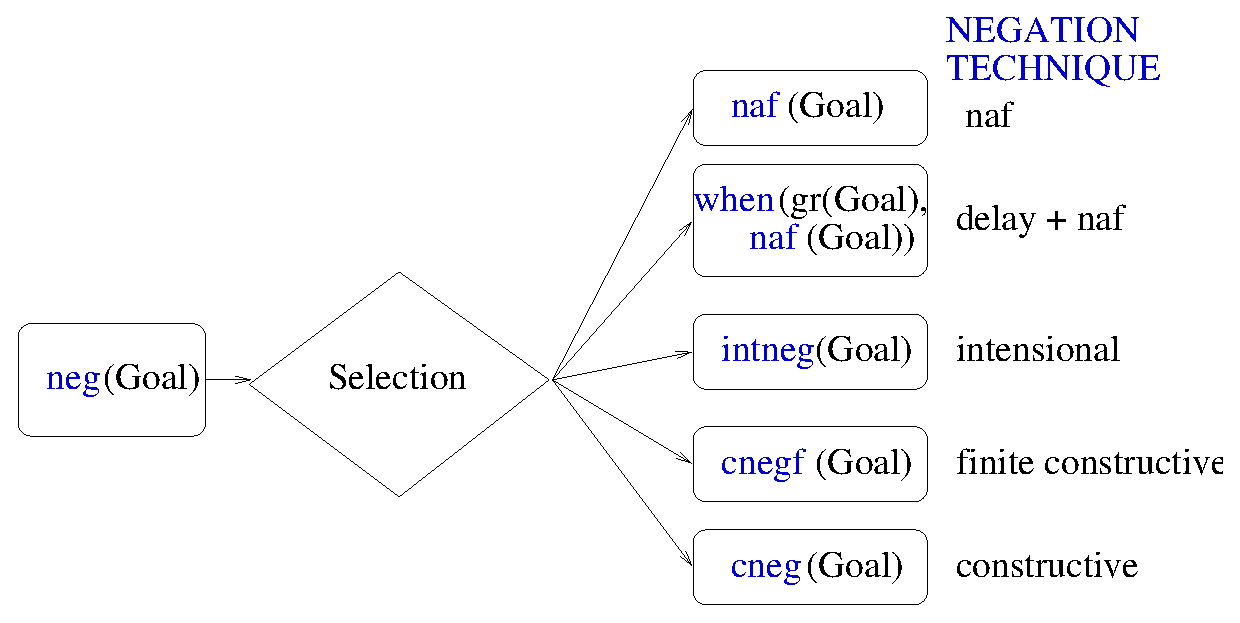
\includegraphics[width=4in]{modules.eps} 
  \end{figure}
\vspace{-0.5cm}
      \begin{itemize}
                \item[{\blue $\bullet$}] Static phase + Dynamic phase
      \end{itemize}

\end{slide}

%%%%%%%%%%%%%%%%%%%%%%%%%%%%%%%%%%%%%%%%%%%%%%%%%%%%%%%%%%%


%%%%%%%%%%%%%%%%%%%%%%%%%%%%%%%%%%%%%%%%%%%%%%%%%%%%%%%%%%%
\maketitle

\end{document} 

%%%%%%%%%%%%%%%%%%%%%%%%%%%%%%%%%%%%%%%%%%%%%%%%%%%%%%%%%%%


